\section{URDAD's Meta Model \label{sec:metamodel}}

URDAD's meta model provides a formal description of URDAD's domain of discourse. It will be used to support the URDAD methodology of requirements specification. A meta model is a ``logical information model that specifies the modeling elements used within another (or the same) modeling notation'' \cite{_ieee_2003}. 

URDAD's meta model formalizes the modeling constructs needed for the specification of service requirements 
and the technology-neutral design of business processes which fulfil such requirements. It is denoted with help of the well-known EMOF/Ecore tool suite, which supports the automatic generation of concrete syntax forms, QVT-based model transformations, as well as the integrated use of the Object Constraint Language (OCL) \cite{_object_2010}. An automatic translation of the meta model into the well-known Web Ontology Language (OWL DL) ontology was done to facilitate automated satisfiability checking (see Section \ref{sec:assessment}).

Our meta model was designed to contain the smallest sufficient set of concepts that describe URDAD's service-oriented analysis and design specifications. In particular the meta model's features capture the above-mentioned decomposition of service requirements with pre- and post-conditions, the specification of non-functional quality requirements, the specification of I/O data types, as well as the specification of service `orchestrations'. The conception of our meta model was influenced by the UML and the Business Process Execution Language (BPEL) in the area of data structure and process specification. One of its underlying assumptions is the internal `statelessness' of the services to be composed; `state' is assumed to be stored in the services' environments.

The URDAD DSL is only a fraction of the size of the UML, yet it includes all core concepts required by the URDAD methodology. In particular it can describe the notion of a responsibility domain, intra-model relationships facilitating traceability, service contracts including pre-conditions and exceptions, service-specific request and result classes, and the separation of the identification of a resource (object or service) from the path to it. Our DSL can even describe a system of parameterised, reusable operational constraints, which are assessed through processes that gather information from their environment. This will be illustrated in the following sub-sections.

%--------------------------
\subsection{The Core of URDAD's Meta Model}

The core module of our meta model captures the concept of an URDAD model as such, i.e.: its model elements and stake holders, responsibility domains, as well as further expressions and annotations as shown in Figure \ref{fig:coreModule}.
\begin{figure}[Htb]
  \centering
  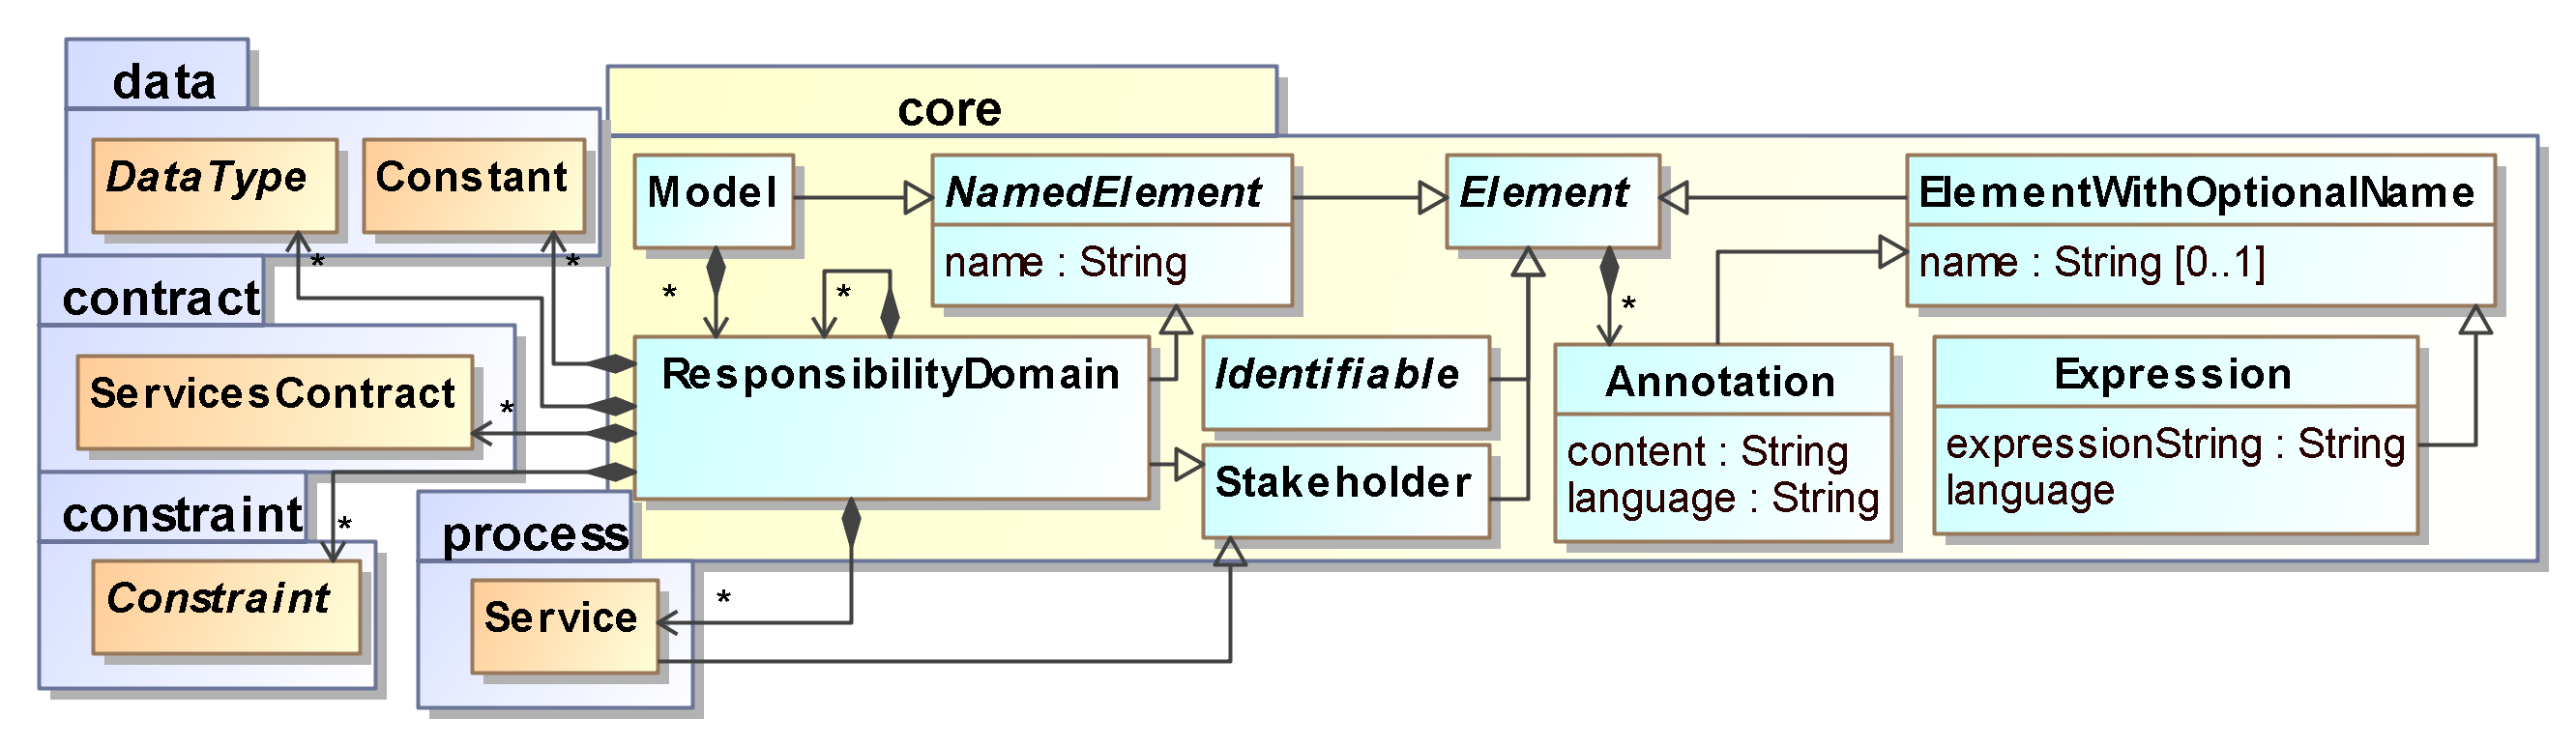
\includegraphics{core}
  \caption{The core elements of URDAD}
  \label{fig:coreModule}
\end{figure}

The picture shows that responsibility domains are assigned to various resources (e.g., persons, systems, modules). A responsibility domain covers a coherent unit of functionality at a particular level of granularity, as previously mentioned. Responsibility domains are pragmatically meaningful groups of service contracts. They also define the boundaries between different levels of granularity. Thereby our notion of `responsibility domain' is similar to the notion of `unity criteria' in \cite{gonzalez_unity_2009}. Technically, responsibility domains are packaging constructs to subsume model elements under a unique name space.

Using tools like EMFText \cite{heidenreich_derivation_2009} one can either generate or specify a textual grammar for a metamodel, and from this grammar both a parser and a language-aware editor (supporting syntax checking and auto-completion) can be generated. In this section we illustrate core aspects of the URDAD DSL through an example encoded in the grammar which we have defined for the language. The textual grammar is meant to be simple and intuitive, enabling requirements specialists to manipulate URDAD DSL - although a graphical editor would ultimately be more suitable.

%-----------------------
\subsection{Constraints}

\todo{Dawid: Consider moving constraints after everything}

The Object-Constraint Language (OCL) has become de-facto standard for specifying constraints across object graphs. However, in a services-oriented approach and in the context of reusable, parameterised constraints the OCL alone is not expressive enough. In particular, the definition of reusable constraints requires support for binding parameters. 

\emph{For example}, assume a constraint that some `Person' must be `registered'. Such a constraint can contribute to pre- or post-conditions of services. Hence, to be able to do so, the person identifier would have to be passed as a parameter to the constraint entity.

Another reason why the URDAD-DSL captures the integration of an additional constraint infrastructure is that in a service-oriented context the actual environmental state is not directly specified, but accessible only via services. In such a context it is not feasible to specify testable conditions via OCL, for OCL is made for 'speaking' about objects, not about their environments.

The specification of constraints must relate to the specification of services that are used to obtain the state information and the associated service request objects. The construction of the related request objects might itself require a process to obtain information from the environment. The URDAD-DSL is suitable for this purpose. OCL (or similar constraint specification languages) can then be used to specify the object constraints that apply to the obtained environmental information.

As it is depicted in Figure \ref{fig:constraintModule}, the constraints module provides the concept of re-usable constraints with standard logical operators to formulate complex constraint expressions.
\begin{figure}[Htbp]
  \centering
  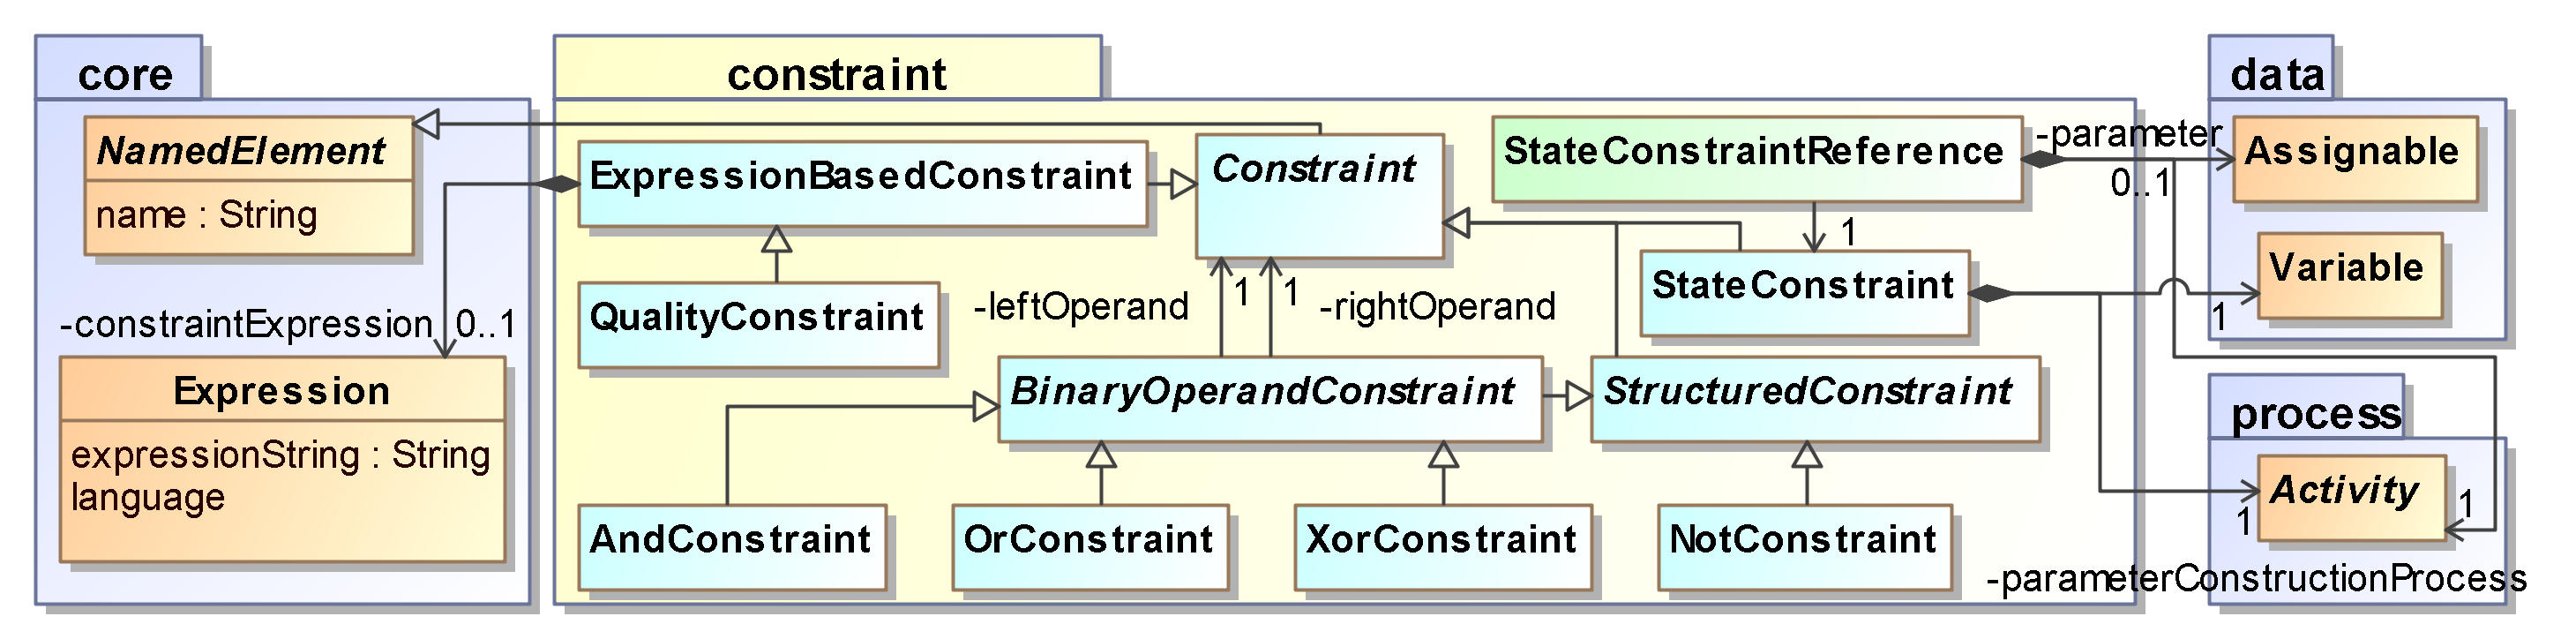
\includegraphics{constraint}
  \caption{The constraint specification elements of URDAD}
  \label{fig:constraintModule}
\end{figure}

The following listing shows an extract of the textual representation of our 'registration' example. It illustrates the specification of a simple parametrised constraint which includes the specification of a process that extracts information from the environment as well as a data constraint to be checked against the such-obtained information.
\tiny \begin{lstlisting}[numbers=left,escapechar=|]
StateConstraint studentEnrolledForPresentation receiving Variable 
  enrollForPresentationRequest ofType EnrollForPresentationRequest
{
  stateAssessmentProcess doSequential
  {
    create Variable getEnrollmentsRequest ofType GetEnrollmentsRequest
    set Query OCL:"getEnrollmentsRequest.presentationIdentifier" equalTo
        Query OCL:"enrollForPresentationRequest.presentationIdentifier"
    requestService getEnrollments with getEnrollmentsRequest yielding
        Variable getEnrollmentsResult ofType GetEnrollmentsResult
  }
  Constraint OCL:"getEnrollmentsResult.enrollments.includes
    (enrollForPresentationRequest.personIdentifier)"
}
\end{lstlisting}\normalsize
\lstset{caption=My Caption,label=my_label}


%----------------------------
\subsection{Service Contracts}

A service contract comprises both functional and non-functional quality requirements. Every requirement is associated with a stakeholder which is either a responsibility domain or another service. Functional service requirements are expressed in terms of the above-mentioned pre- and post-conditions, together with exception rules for the case that any pre-condition is not fulfilled. This is depicted in Figure \ref{fig:metamodel-3}.
\begin{figure}[Htbp]
  \centering
  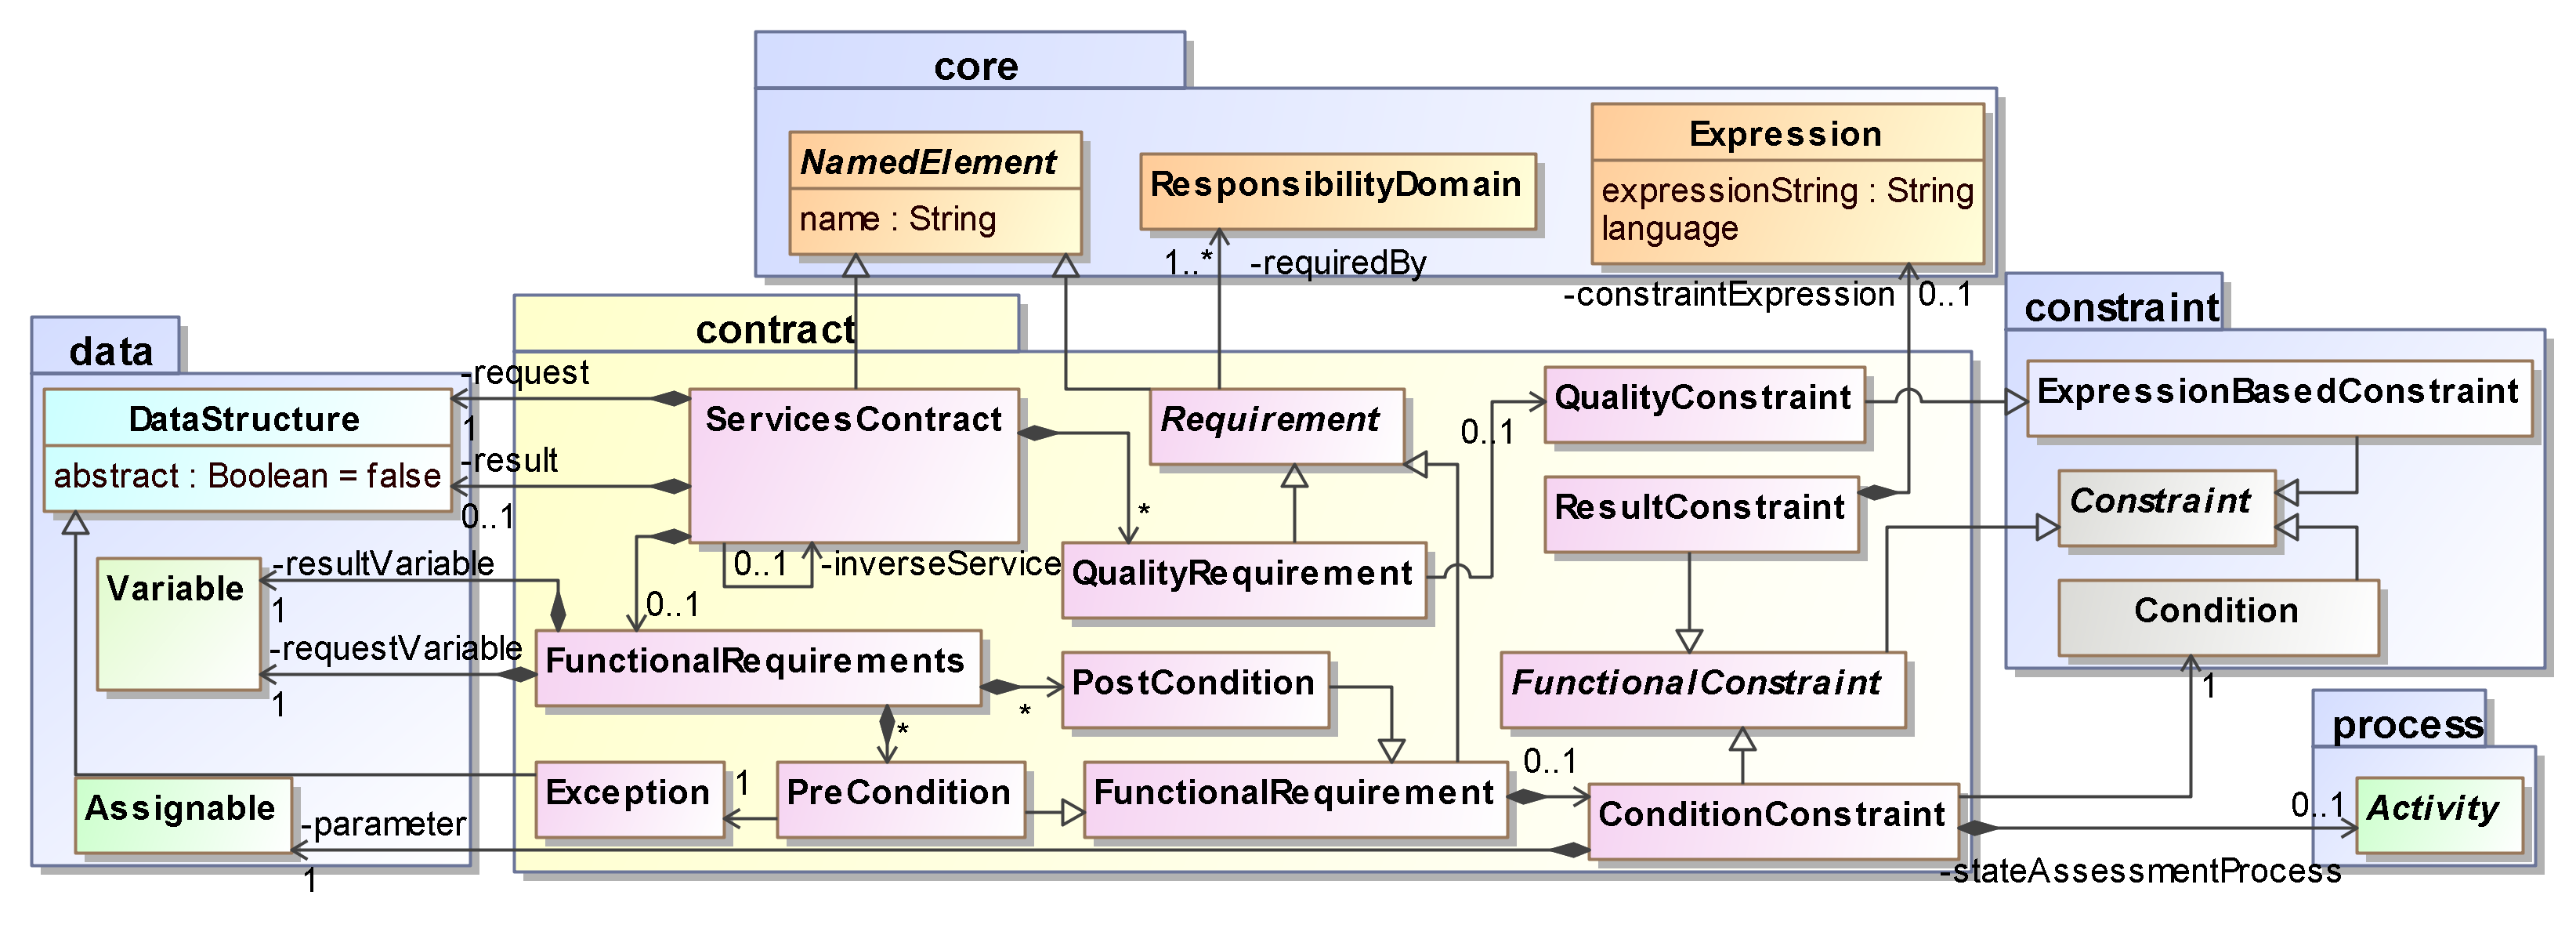
\includegraphics{contract}
  \caption{The contract specification elements of URDAD}
  \label{fig:contractModule}
\end{figure}

A post-condition can specify either the computational output of a service, or its \emph{side effects} on its environment. Due to a service potentially creating a lasting change to its environment, the URDAD-DSL allows the designation of inverse services through which these lasting effects can be reversed. Explicit post-conditions thus also help to specify such undo-services.

A service contract specifies a single service request object that contains information pertaining to the request and a single result object, which contains the information associated with the result of the executed service. The data structures for these request and result objects are service-specific and are not meant to be reused (though their components, which are domain objects, are most likely to be reused). Below we illustrate the specification of a service contract in our URDAD DSL grammar.
\tiny \begin{lstlisting}[numbers=left,escapechar=|]
ServiceContract enrollForPresentation
{
   FunctionalRequirements receiving Variable enrollForPresentationRequest 
      ofType EnrollForPresentationRequest
   {
      PreCondition enrollmentPrerequisitesMet
         requiredBy (TrainingRegulator Student) 
         raises EnrollmentPrerequisitesNotSatisfiedException
         checks constraint enrollmentPrerequisitesForPresentationMet
         with ValueOf enrollForPresentationRequest
      PostCondition enrollmentProcessPerformed
         requiredBy (Student Client TrainingRegulator)
         ensures constraint studentEnrolledForPresentation 
         with ValueOf studentEnrolledRequest constructedUsing doSequential
         {
            create Variable studentEnrolledRequest ofType StudentEnrolledRequest
            set Query OCL:"studentEnrolledRequest.personIdentifier" equalTo
                Query OCL:"enrollForPresentationRequest.personIdentifier"                            
            set Query OCL:"studentEnrolledRequest.presentationIdentifier" equalTo
                Query OCL:"enrollForPresentationRequest.presentationIdentifier"                            
         }  
      PostCondition invoiceIssued ...
    }            
    Request DataStructure EnrollForPresentationRequest 
    {
       has identification presentationIdentifier identifying Presentation
       has identification studentIdentifier identifying Person
       has component clientIdentifier ofType LegalEntity         
    }
    Result DataStructure EnrollForPresentationResult 
    {
       has component proofOfEnrollment ofType ProofOfEnrollment
       has component invoice ofType Invoice
       has component studyGuide ofType StudyGuide
    }
}
\end{lstlisting}\normalsize

%--------------------------
\subsection{Data Structures}

The data module of the URDAD meta model is depicted in Figure \ref{fig:metamodel-4}. It allows for an object-oriented approach to data structure specification, similar to UML class descriptions. For the purpose of this paper it it not necessary to go into the finer details of this package which descibes, basically, what kind of data two services can communicate amongst each other.
\begin{figure}[Htbp]
  \centering
  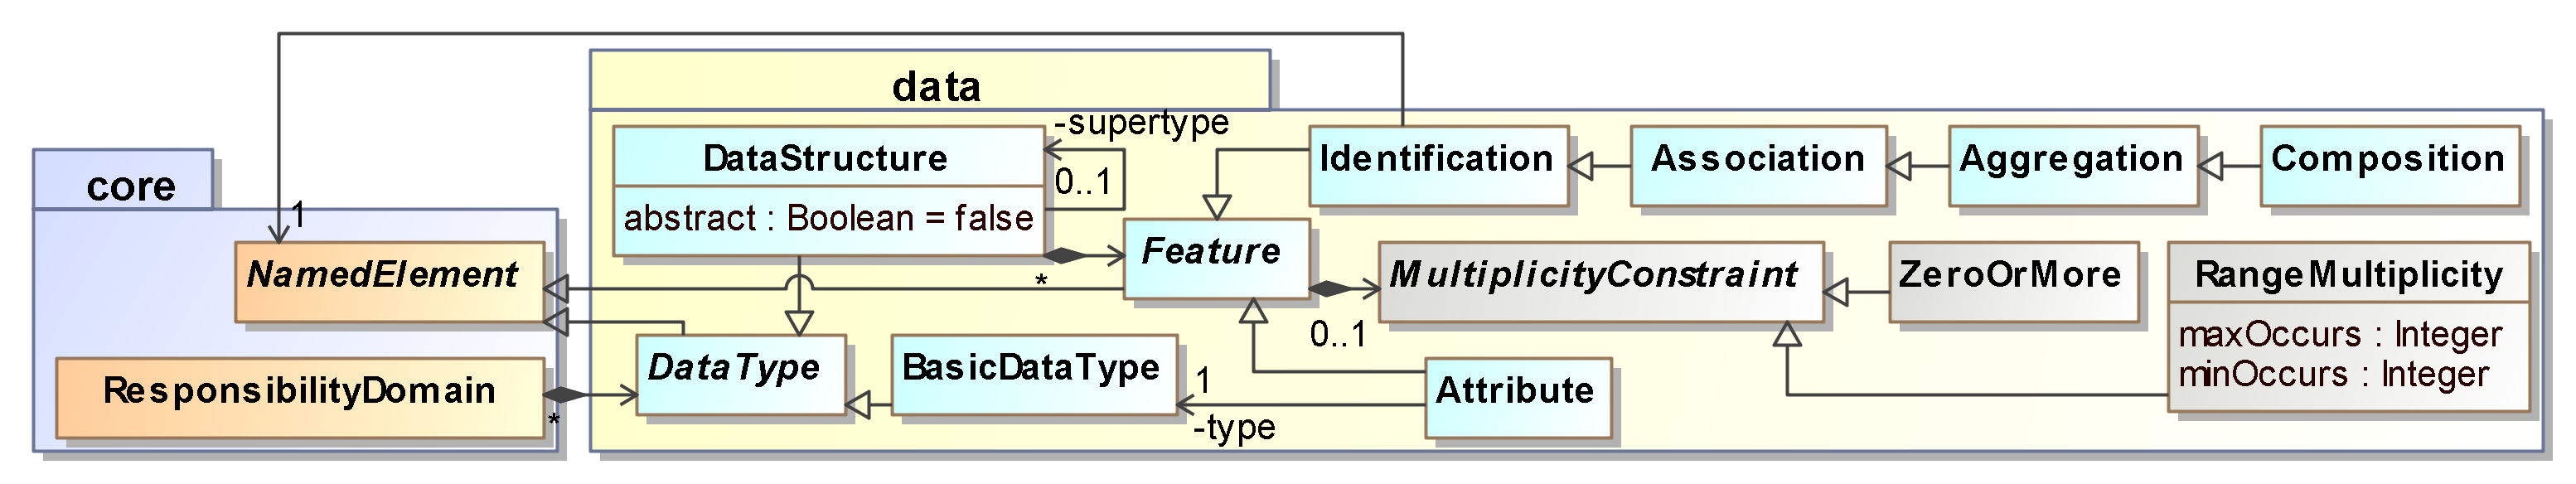
\includegraphics{data}
  \caption{The data definition elements of URDAD}
  \label{fig:dataStructureModule}
\end{figure}

\todo{Add identification vs association in a more compact form}

%--------------------
\subsection{Processes}

The process package of the URDAD meta model describes the concept of a service as a concrete unit of functionality in fulfillment of its service contract. In this context, traceability is suported by `satisfaction' links as in \cite{ramesh_toward_2001}). A service is thus conceptually associated with its own local variables, the validation of a pre-condition and/or the fulfilment of a post-condition, the handling of an exception raised by a sub-service, the raising of an exception at its own level, or the return of a computational result. Figure \ref{fig:processModule} shows this section or the URDAD meta model.
\begin{figure}[Htbp]
  \centering
  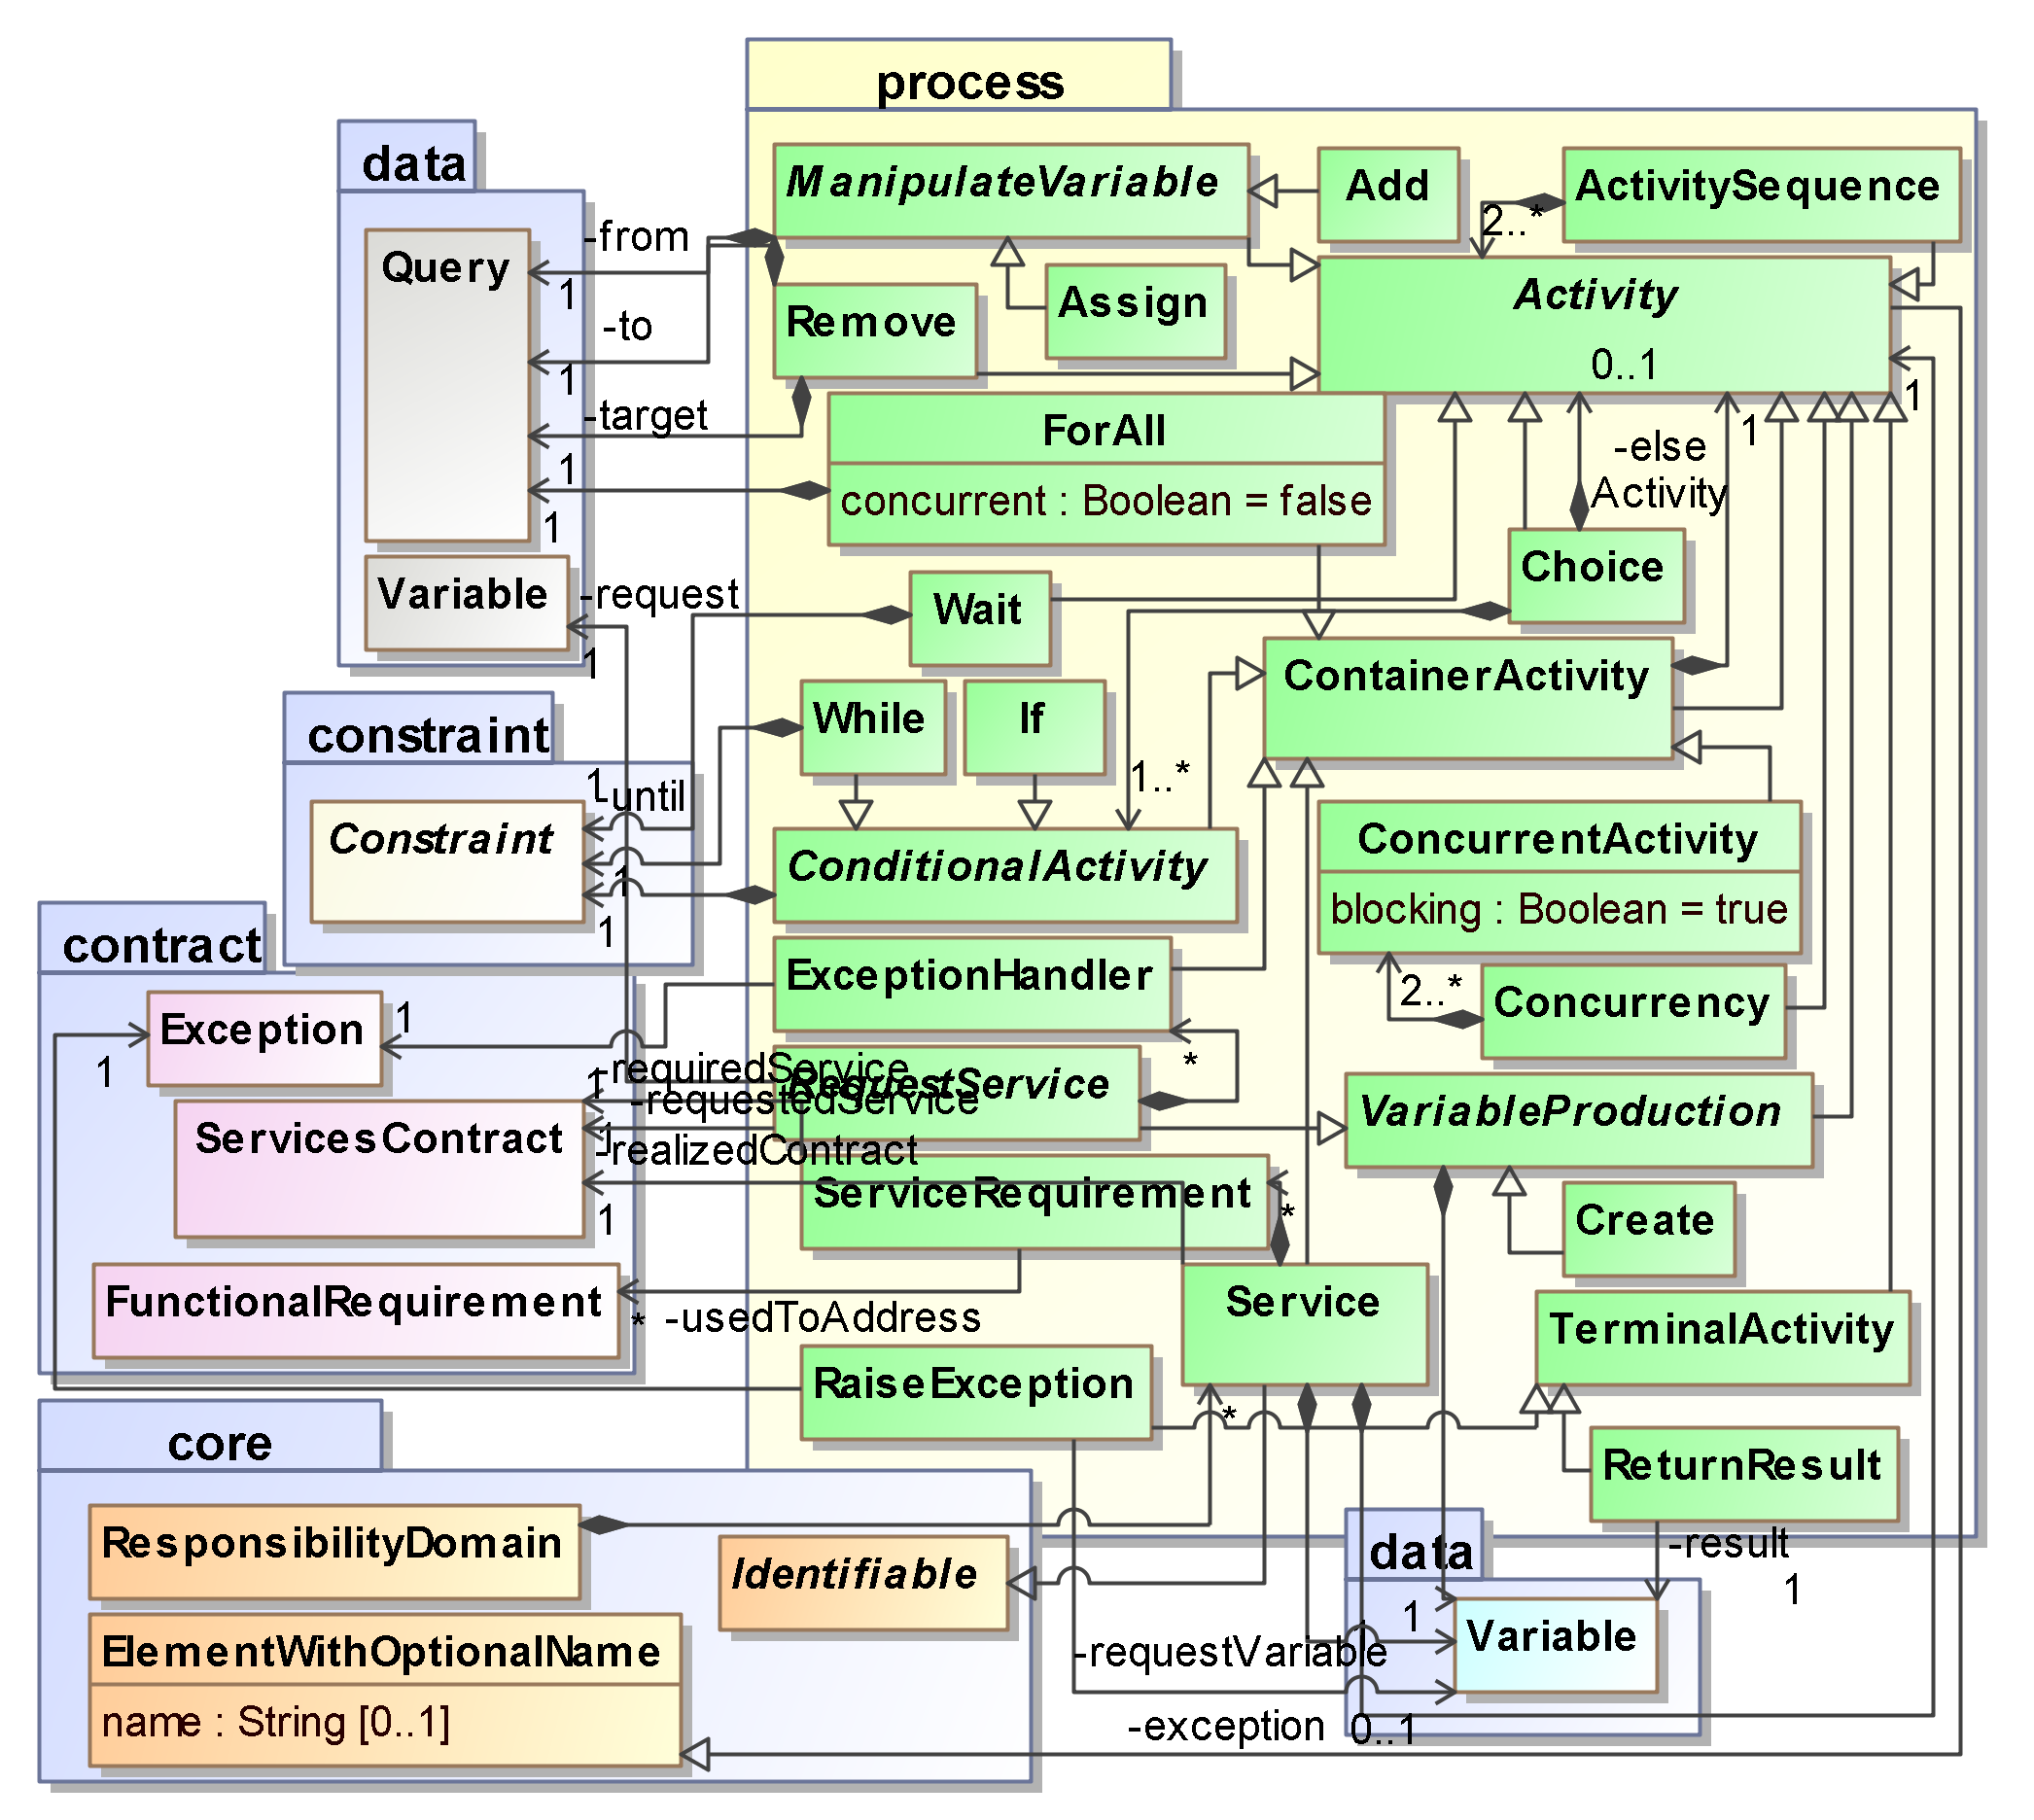
\includegraphics{process}
  \caption{The process definition elements of URDAD}
  \label{fig:processModule}
\end{figure}

The URDAD methodology enforces `decoupling' through service contracts. This is reflected in the URDAD meta model by associating satisfaction links as well as service requests to service contracts (instead of to concrete services). Also note that URDAD methodology assumes that the concrete services will either be implemented through model-transformations (MDE), or will be provided through the underlying infrastructure (e.g., run-time environments). Therefore, the finer details of service implementations are not represented in the our technology-neutral URDAD models. The following listing shows how a service contract is denoted in the grammar of our URDAD DSL.

\tiny \begin{lstlisting}[numbers=left,escapechar=|]
Service enrollForPresentationImpl realizes enrollForPresentation 
 receiving Variable enrollForPresentationRequest ofType EnrollForPresentationRequest
{
  use checkStudentSatisfiesEnrollmentPrerequisites 
    toAddress (enrollmentPrerequisitesMet)
  use issueInvoice toAddress (financialPrerequisitesSatisfied invoiceIssued) 
  use performEnrollment toAddress (invoiceIssued)
   
  doSequential
  {
    create Variable checkStudentSatisfiesEnrollmentPrerequisitesRequest 
      ofType CheckStudentSatisfiesEnrollmentPrerequisitesRequest               
    set Query OCL:"enrollForPresentationRequest.studentIdentifier" equalTo 
        Query OCL:"checkEnrollmentPrerequisitesRequest.studentIdentifier"
    set Query OCL:"enrollForPresentationRequest.presentationIdentifier" equalTo
        Query OCL:"checkEnrollmentPrerequisitesRequest.presentationIdentifier"
                     
    requestService checkStudentSatisfiesEnrollmentPrerequisites 
      with checkStudentSatisfiesEnrollmentPrerequisitesRequest 
        yielding Variable checkStudentSatisfiesEnrollmentPrerequisitesResult
          ofType CheckStudentSatisfiesEnrollmentPrerequisitesResult
    choice
    {
      if Constraint enrollmentMeetsPrerequisitesMet 
        OCL:"checkStudentSatisfiesEnrollmentPrerequisitesResult.
                enrollmentPrerequisitesMet = true"
        doSequential
        {
          ...
          requestService issueInvoice with issueInvoiceRequest 
            yielding Variable issueInvoiceResult ofType IssueInvoiceResult
          {
            on FinancialPrerequisitesNotSatisfiedException 
              raiseException FinancialPrerequisitesNotSatisfiedException
          }
	      ...
          requestService performEnrollment with enrollRequest 
            yielding Variable performEnrollmentResult ofType PerformEnrollmentResult
          
          create Variable enrollForPresentationResult 
            ofType EnrollForPresentationResult
          set Query OCL:"issueInvoiceResult.invoice" equalTo
              Query OCL:"enrollForPresentationResult.invoice"
          ...                       
          returnResult  enrollForPresentationResult
        }
      else raiseException EnrollmentPrerequisitesNotSatisfiedException
    }
  }
}                 
\end{lstlisting}\normalsize

 
